%growth rates not sig changed 
%v shear from thin dust layers are overwhelmed by 
\section{Discussion}\label{discussion}


{\bf

%pros and cons 
%energy analogy not restricted to term vel approx 
%spurious modes

\subsection{Applications and limitations}

The main application we envision for the dusty/adiabatic gas analogy 
is to develop physical interpretations of dust-gas drag instabilities; and to find 
dusty analogs of pure gas instabilities in protoplanetary disks, 
which is discussed in \S\ref{dust_analogs}. One can also exploit the similarity to adapt existing
hydrodynamic codes to simulate dusty protoplanetary disks (see \S\ref{dust_sims}). 

It is important to keep in mind the assumptions 
used to develop our thermodynamic model of dusty gas. 
The terminal velocity approximation, $\bm{v}_\mathrm{d} -
\bm{v}_\mathrm{g} = \tstop \nabla P /\rhog$, was employed from the
outset. 
%It assumes  
%the dust-gas relative drift $\bm{v}_mathrm{d} - \bm{v}_\mathrm{g} =
%\tstop \nabla P /\rhog$ 
This is applicable to small particles with short stopping times and
strongly coupled to the gas. Generally we require $\tstop$ to be the
shortest timescale in the physical problem. For  
example, to study dust settling, we require $\tstop \ll
t_\mathrm{settle}\sim 1/\tstop\OmK^2$, or 
$\tstop\OmK \ll 1$. 

%However, the validity of the simplified one-fluid equations may be
%problem-dependent, and not just on the terminal velocity 
%approximation. 

However, the validity of the terminal velocity approximation may not
only depend on $\tstop$. The value of the dust gas-ratio and the
problem itself may also be important. 
%You can decide if this is a relevant improvement, and whether to
%include. 
For example, Table \ref{si_compare} shows the dust-rich
`linA' mode and dust-poor `linB' mode of the streaming instability
have the same $\tstop$, but the former is accurately captured by the
simplified equations, while the latter is not.  This suggests that for
the streaming instability the simplified equations is better suited
for $\rhod/\rhog>1$. The simplified equations also contain spurious
modes in certain limits (see \S\ref{spurious_epi}). 

%Ultimately,
                                %one must 
                                %c heck against the full equations.  

Note that our thermodynamic interpretation of dust-gas drift does
\emph{not} actually depend on the terminal velocity approximation.   
Once the gas equation of state is fixed and the true energy equation deleted, 
the dust continuity equation can be converted to a new effective energy equation. 
As an example, for strictly isothermal dusty gas we obtain   
\begin{align}
\frac{DP}{Dt} = - P\nabla\cdot\bm{v} +
c_s^2\nabla\cdot\left[\fdust\left(1-\fdust\right)\rho\left(\bm{v}_\mathrm{d}
    - \bm{v}_\mathrm{g}\right)\right]. \label{no_term_vel}  
\end{align}
This equation does not use
the terminal velocity approximation (which gives
Eq. \ref{eff_energy}). Evaluating the right-hand-side generally 
requires solving an evolutionary equation for $\bm{v}_\mathrm{d} - 
\bm{v}_\mathrm{g}$ \citep{laibe14}. Nevertheless,
Eq. \ref{no_term_vel} shows that dust-gas relative drift can be
interpreted as a heat flux within the dust-gas mixture. Thus, even 
without the terminal velocity approximation we can 
regard the dusty-gas as a single ideal fluid subject to cooling.   
}

\subsection{Generalization to locally polytropic disks}\label{gen_poly}

%\subsubsection{Locally polytropic disks}
We can extend the dusty/adiabatic gas correspondence to 
other fixed equations of state. As an example, consider the locally
polytropic disk 
\begin{align}
  P = K(r,z)\rhog^{\Gamma}, 
\end{align}
where $K$ is a prescribed function and $\Gamma$ is the constant
polytropic index. Then eliminating $\tepsilon$ from the dust equation
\ref{dusteq} gives 
\begin{align}\label{poly_energy}
  \frac{D P}{D t} &= - \Gamma P\nabla\cdot\bm{v}  + P \bm{v}\cdot\nabla
  \ln{K} + \frac{\Gamma P}{\rhog}\nabla\cdot\left(\tepsilon\tstop\nabla
  P\right). 
%+ \mathcal{C},\\
%  \mathcal{C}& = \frac{\Gamma P}{\rhog}\nabla\cdot\left(\tepsilon\tstop\nabla
%  P\right).
\end{align}
Thus the dusty gas behaves like a pure gas with adiabatic index
$\Gamma$. The entropy is given by 
\begin{align}
  \seff = \ln{\left[K^{1/\Gamma}(r,z)\left(1 - \tepsilon\right)\right]}.  
\end{align}
The results of \S\ref{iso_perfect}---\ref{dust_work} remain valid for the strictly 
polytropic disk with $K=$constant, while one sets $c_s^2\to K$ in
\S\ref{dusty_vsi_int}. 
%When $K$ is constant, the corresponding Solberg-Hoiland criteria for
%axisymmetric stability may be obtained from that in standard adiabatic 
%hydrodynamics \citep[e.g.][]{tassoul78} by
%using this definition of entropy in
%Eqs. \ref{dusty_solberg1}---\ref{dusty_solberg2}. 




%In particular, we will explore whether this can surpress the suprious
%modes discussed in Appendix \S\ref{spurious_epi}. 

%stratified case require more boundary conditions 



\subsection{Dusty analogs of other gaseous instabilities} \label{dust_analogs} 

%gi
%rwi 

\subsubsection{Classic gravitational instabilities} %vertical structure 
The addition of dust enhances gravitational
instability (GI) because dust particles contribute to the
total disk mass but not thermal pressure, which effectively lowers the
disk temperature \citep[][]{thompson88,shi13}. For typical dust-loading 
$\tepsilon, Z\ll1$, this effect is unimportant. However, if $\epsilon$ is
large (e.g. due to dust settling) then the reduced temperature
$\widetilde{T}~=~T(1 - \tepsilon)$ may be lowered to enable instability.  

As noted in \S\ref{loc_iso_eos}, dust settling causes 
$\widetilde{T}$ to \emph{increase} away from the midplane. This contrasts
to previous studies of GI in vertically stratified disks
 where the temperature decreases
from the midplane \citep[e.g.][]{mamat10, kim12,lin14c}. 
While we expect only the total surface density and
characteristic temperatures are relevant to stability  
\citep{toomre64}, a non-trivial vertical temperature
structure, induced by dust, may modify the vertical structure of 3D
waves and unstable modes. 

Another potential connection to previous results for gas disks is  
gravito-turbulence. Cooling, self-gravitating gaseous disks 
sustain a turbulent state where shock heating due to gravitational 
instabilities are balanced by radiative cooling 
\citep{gammie01}. Since dust-gas drift appears as a diffusion or 
cooling in our framework (Eq. \ref{eff_energy}), it may be conceivable
to have `dusty gravito-turbulence'. As self-gravity increases the
local density, the associated pressure maxima attract dust-particles,
but the back-reaction onto the gas may try to flatten the pressure
bump \citep{taki16}, thus enabling a quasi-steady state. 

%see also
%\S\ref{loc_iso_eos}
%We thus expect the standard Toomre
%parameter to be modified to $Q = c_s\sqrt{1-\tepsilon}\Omega/\pi
%G\Sigma$. 

\subsubsection{Rossby wave instability}
The Rossby wave instability (RWI) is a non-axisymmetric, 2D shear
instability that operates in thin disks when it has radial structure
\citep{lovelace99,li00}. These studies consider adiabatic pure gas and 
show instability is possible if there is an extremum in the generalized
potential vorticity 
%\begin{align}
 $\mathcal{V}_\mathrm{g} =
 \kappa^2\mathcal{S}_\mathrm{g}^{-2/\gamma}/2\Omega\Sigma_\mathrm{g}$, 
%\end{align} 
where $\mathcal{S}_\mathrm{g} = P/\Sigma_\mathrm{g}^\gamma$ is essentially
the gas entropy. Here $P$
should be interpreted as the vertically integrated pressure. The
non-linear result of the RWI is vortex formation \citep{li01}. 

The dusty/adiabatic gas analogy imply the condition for RWI in a
polytropic dusty gas disk is an extremum   
\begin{align}
  \mathcal{V} =
  \frac{\kappa^2}{2\Omega\Sigma}\frac{1}{K^{2/\Gamma}}\left(1+
    \frac{\Sigma_\mathrm{d}}{\Sigma_\mathrm{g}}\right)^2.    
\end{align}
Thus RWI may also be triggered by extrema 
in the dust-to-gas ratio, e.g. narrow dust rings/gaps. This may lead 
to direct formation of dusty vortices, as opposed to dust-trapping by  
a pre-existing gas vortex \citep{barge95,lyra13}.  

%{\bf so may it's not vortex formation then dust-trapping. could just
%  form dusty vortices in one go}

%gap edges. thin dust rings. 

\subsubsection{Convective overstability}
The `convective overstability' (ConO) was discovered in pure gas, non-adiabatic, unstratified disk models    
where the radial buoyancy frequency is such that $N_r^2\equiv
F_r\p_rS/C_P  < 0 $ and cooling times $t_\mathrm{cool}\sim \OmK^{-1}$. This
combination leads to growing epicycles
\citep{klahr14,lyra14,latter16}.     
%with 
%growth rate $\propto  -N_r^2$ 
% Indeed, the effective radial buoyancy frequency in our dusty disk 
% with negligble background density gradient is unstable, 
% \begin{align}
%   N_r^2 \equiv -\frac{1}{\rho}\frac{\p P}{\p r}\frac{\p S_\mathrm{eff}}{\p r} =
%   -\frac{\rho}{P}F_r^2<0.  
% \end{align}

%The disk structure required for ConO might be realized in a locally
%isothermal dusty disk. 

Now consider a strictly isothermal dusty disk where the relevant 
entropy is dust-induced, $\seff =-\ln{(1+\rhod/\rhog)}$. 
%The dusty/adiabatic gas
%analogy implies the replacement $S\to\seff = -\ln{(1+\rhod/\rhog)}$ in
%$N_r$. 
Since $F_r\propto -\p_rP > 0$ in typical disk models, ConO would
require $\p_r\seff<0$, implying the dust-to-gas ratio increases
\emph{outwards}. This might be realized at special radial locations in 
protoplanetary disks, such as planet gaps. Dust-settling itself may
also lead to the mid-plane dust-to-gas ratio to increase outwards
\citep{takeuchi02}. 

%fact, the typical disk models used to study the streaming
%instability have zero background radial density gradient, in which
%case  $N_r^2= -\rho F_r^2/P < 0$.   

Isothermal disks have $\tcool=0$, so the pure gas ConO cannot
exist. However, we have shown that dust-gas drag provides an effective
energy source/sink to the mixture (\S\ref{energy_analogy}). It would be
interesting to explore whether or not dust-gas drag can play the role
of cooling to enable a `dusty convective 
overstability'. 

%Furthermore, 
%the effective radial buoyancy frequency in our dusty disk  
%with negligble background density gradient is unstable, 
%\begin{align}
%   N_r^2 \equiv -\frac{1}{\rho}\frac{\p P}{\p r}\frac{\p S_\mathrm{eff}}{\p r} =
%   -\frac{\rho}{P}F_r^2<0.  
% \end{align}



% One might then think of the streaming instability as a dusty relative
% to the convective  overstability. Explicit solutions in the small
% $\tstop$ limit show that streaming instability growth rates are
% also $\propto |N_r^2|$  \citep{jacquet11}, as is for the convective
% overstability \citep{lyra14,latter16}. Furthermore, both instabilities require
% finite effective cooling times, and both require $k_z\neq0$. 
% %{\bf note: si osc freq not too small compared to kappa} 

% However, the convective overstability is most unstable at $k_x=0$
% \citep{lyra14}  whereas the streaming instability growth rate is maximized at finite $k_x$
% \citep{youdin05a}. 


\subsubsection{Zombie vortices}

The `zombie vortex instability' (ZVI) is a non-axisymmetric,
non-linear instability discovered in pure gas disks
\citep{marcus15,umurhan16d}. It operates by having finite-amplitude perturbations
exciting `critical layers',  where the intrinsic wave frequency of the
perturbation matches the local vertical buoyancy frequency 
\citep{marcus13}. These critical layers roll 
up into vortices, exciting further critical layers. The process
repeats itself and the result is an array of vortices. 

Since the necessary physical ingredient for the ZVI is vertical
buoyancy, it requires an almost purely adiabatic gas with long cooling times ($\tcool\OmK\gg
1$). This limits its applicability in typical protoplanetary disks to 
$\lesssim 1$AU \citep{lesur16, malygin17}. However, this consideration
assumes a dust-free disk as far as the dynamics is concerned. 

On the other hand, we have show that dust-loading induces an effective
buoyancy even in isothermal disks. It is thus natural to ask whether or not
the required adiabatic conditions for ZVI can be realized through
dust-loading (specifically a vertical gradient in the dust-to-gas ratio), 
and thus produce `dusty ZVI'. This may allow the zombie 
vortices to develop $\gtrsim 1$AU in PPDs. 

\subsection{Implications for numerical simulations}\label{dust_sims}
{\bf The one-fluid model with the terminal velocity approximation, Eq. \ref{masseq}---\ref{momeq}, 
has been applied to simulate dusty protoplanetary disks \citep{dipierro15,ragusa17}. These studies 
explicitly evolve the dust density.  
}

{\bf However, the dusty/adiabatic gas equivalence identified in this paper
means that one need not implement a separate module for simulating the dust component in
locally isothermal/polytropic gas. The standard energy equation substitutes for the dust continuity 
equation. Thus pure gas dynamic codes can be used to simulate protoplanetary dusty disks. 
} %means that pure 
%gas dynamics codes can be applied to simulate locally 
%isothermal/polytropic dusty gas. One need not implement a separate 
%equation for the dust component: 
%for strictly isothermal or polytropic gas perfectly-coupled to dust:  
% the standard energy equation substitutes for the dust continuity
%equation. 
When {\bf the sound-speed} $c_s$ (or $K$) is not constant and/or the dust-gas coupling is imperfect, $\tstop\neq0$, one
should add corresponding source terms in the energy equation
(e.g. Eq. \ref{poly_energy}). 
The source term associated with dust-gas drag, $\mathcal{C}$, is 
analogous to radiative diffusion \citep{price15} or thermal 
conduction, which is also common in modern hydrodynamics codes.       

We have taken advantage of the dusty/adiabatic gas equivalence to 
convert the popular
\textsc{Pluto}\footnote{\url{http://plutocode.ph.unito.it/}}      
hydrodynamics code \citep{mignone07} into a dusty gas dynamics code appropriate for
simulating protoplanetary disks coupled to small dust. {\bf In fact,
  our code is unaware of the fact that it is modeling dusty gas.} 
We will apply 
this modified code ---d\textsc{Pluto}--- to study dusty disk-planet interaction (Lin et al., 
in preparation). 
Preliminary results {\bf show our approach} %indicate the simplified one-fluid 
reproduce features such as dusty rings associated with 
planet-induced gaps similar to that obtained from explicit two-fluid
simulations \citep[e.g.][]{dong17}. 

% \subsection{Higher order corrections}
% {\bf notes for self. maybe exclude in final. maybe move into appendix}

% The simplified one-fluid formulation, 
% Eqs. \ref{masseq}---\ref{tempeq}, can 
% produce spuriously-growing modes with frequency $|\sigma|\gtrsim
% \Omega$ (see Appendix \S\ref{spurious_epi}). This 
% results from neglecting terms of $O(|\bm{v}_\mathrm{d}-\bm{v}_\mathrm{g}|^2)$ after converting
% the full two-fluid equations to the one-fluid formulation. The full
% one-fluid equations 
% %is significantly more complex than our 
% %model \cite[e.g.][]{laibe14}. It 
%  includes an evolutionary equation for $\widetilde{\bm{v}}\equiv\bm{v}_\mathrm{d}-\bm{v}_\mathrm{g}$, which has no
%  hydrodynamic counter-part \citep{laibe14}. However, it is
%  still possible to improve upon 
%  the first-order formulation whilst retaining similarilty to  
%  standard hydrodynamics.  
% %without having the complexity of the full equations 

% The full one-fluid equations of motion includes the acceleration term 
% \begin{align}
% %\left.\frac{D\bm{v}}{Dt}\right|_\mathrm{add} = 
% %\bm{a} =  
% -\frac{1}{\rho}\nabla\cdot\left(\frac{\rhod\rhog}{\rho}\widetilde{\bm{v}}\otimes\widetilde{\bm{v}}\right) 
% \equiv  \frac{1}{\rho}\nabla\cdot \bm{T} 
% \end{align}
% \citep{youdin05a}, 
% where $\bm{T}$ is an effective stress tensor. 
% In the terminal velocity
% approximation with $\widetilde{\bm{v}} = \tstop 
% \nabla P/\rhog$, we have 
% \begin{align}
% \bm{T} = - \frac{\epsilon\tstop^2}{\rho}\nabla P \otimes \nabla P.
% \end{align}
% If we define 
% \begin{align}
%   \bm{g} \equiv \sqrt{4\pi G \epsilon \rho} \frac{\nabla P}{\rho}
%   \tstop,\label{effective_g} 
% \end{align}
% then
% \begin{align}
% \bm{T} = - \frac{1}{4\pi G} \bm{g}\otimes\bm{g}, \label{effective_gstress}
% \end{align}
% %{\bf tensor virial theorems?}
% which is just the anisotropic part of the  
% gravitational stress tensor in self-gravitating hydrodynamics 
% \citep{lynden-bell72}.

%  However, unlike self-gravity, where $\bm{g}$ is
% determined through the Poisson equation; here $\bm{g}$ is directly
% related to $P$ (Eq. \ref{effective_g}), which itself obeys an 
% evolutionary equation (Eq. \ref{eff_energy}). 
% Nevertheless, Eq. \ref{effective_g}---\ref{effective_gstress}
% show that correlations in  pressure gradients lead to 
% momentum transport of the mixture as a whole. This is similar to Reynolds stresses in
% a turbulent disk \citep{balbus99}. In particular, 
% outwards angular momentum transport requires $\p_rP\p_\phi P > 0$.    

% In a following paper we will include $\bm{T}$ in the one-fluid
% equations and futher explore the analogy between dusty-gas and viscous
% hydrodynamics. 


% \subsection{New dust-drag
%   instabilities}\label{dust_as_thermo} 

% %{\bf vsi enabled by drag? slipping between dust and gas reduces
%  % effective buoyancy}

% As described in \S\ref{dust_work}, 
% the physical cause of dust-drag instabilities is a phase lag between
% the pressure and density response in a dusty gas\footnote{
% In fact, we expect a phase difference between pressure and the total
% density  whenever $\tstop\neq0$; not just $\tstop\OmK\ll 1$ as 
% considered in this work. This is simply because of the finite
% relaxation time required for dust to respond to gas, and vice versa. 
% An effective energy equation in the form of Eq. \ref{eff_energy} can
% still be obtained for general $\tstop$. The
% heat flux $\bm{F}$ in the cooling function $\mathcal{C}$ is determined
% through solution to the relative velocity $\Delta \bm{v} =
% \bm{v}_\mathrm{d}-\bm{v}_\mathrm{g}$ \citep{youdin05a,laibe14}.  We
% thus expect the `pressure-density lag' interpretation of dust-drag 
% instabilities to be generally applicable.}. 
% This may be used to re-interpret the streaming instability or to
% understand other dusty instabilities. For example,
% \cite{loren15,loren16} have recently discovered a new axisymmetric 
% instability in their two-fluid numerical simulations of dusty
% protoplanetary disks. They find it leads to the formation of
% `toroidal vortices'. 

% %give numerical example 
% We have applied our one-fluid stability analysis to find unstable modes  
% similar to that described by \cite{loren15}. We use the same
% parameters reported by them as follows. 
% %we set $p=q=0$, which eliminates VSI and minimizes streaming
% %instabilities as there is no radial pressure gradient at the disk
% %midplane.   
% The total metalicity is $Z=0.01$ and the dust scale-height $H_\mathrm{d} =
% 0.4H_\mathrm{g}$, giving a maximum dust-to-gas ratio
% $\mathrm{max}(\epsilon) = 0.025$. The midplane stopping time is 
% $t_\mathrm{s0}=0.02\OmK^{-1}$. The gas disk parameters are $(p,q,
% \hgas) =(-1.5, -1,0.05)$.  We set $k_x = \pi/H_\mathrm{d}$.      

% Fig. \ref{compare_eigenvals_ts0d02} shows the unstable modes found for
% this setup. We find the usual VSI modes, here with $\omega> 3\hgas\OmK,\, s<
% 0.2\hgas\OmK$. However, we also find modes with $\omega<s$. One of these,
% marked by the blue asterisk, has 
% frequency 
% \begin{align*}
% \sigma = (0.3631\ii - 0.1251)\hgas\OmK. 
% \end{align*}
% This growth rate corresponds to $8.8$ orbits, comparable to the $12$
% orbits reported by \citeauthor{loren15}. We visualize this mode in
% Fig. \ref{result2d_loren}. We find this mode 
% persists when $q=0$, so it is not the VSI. 
% Using Eq. \ref{streaming_dispersion} with the above parameters,  
% we also estimate a much smaller growth 
% rate for the streaming instability of 
% $O(10^{-3}\hgas\OmK)$, We thus also rule out
% SI, as did \citeauthor{loren15}. However, the mode disappears with $\tstop=0$, so it \emph{is}
% associated with finite dust-gas drag. 

% \begin{figure}
%   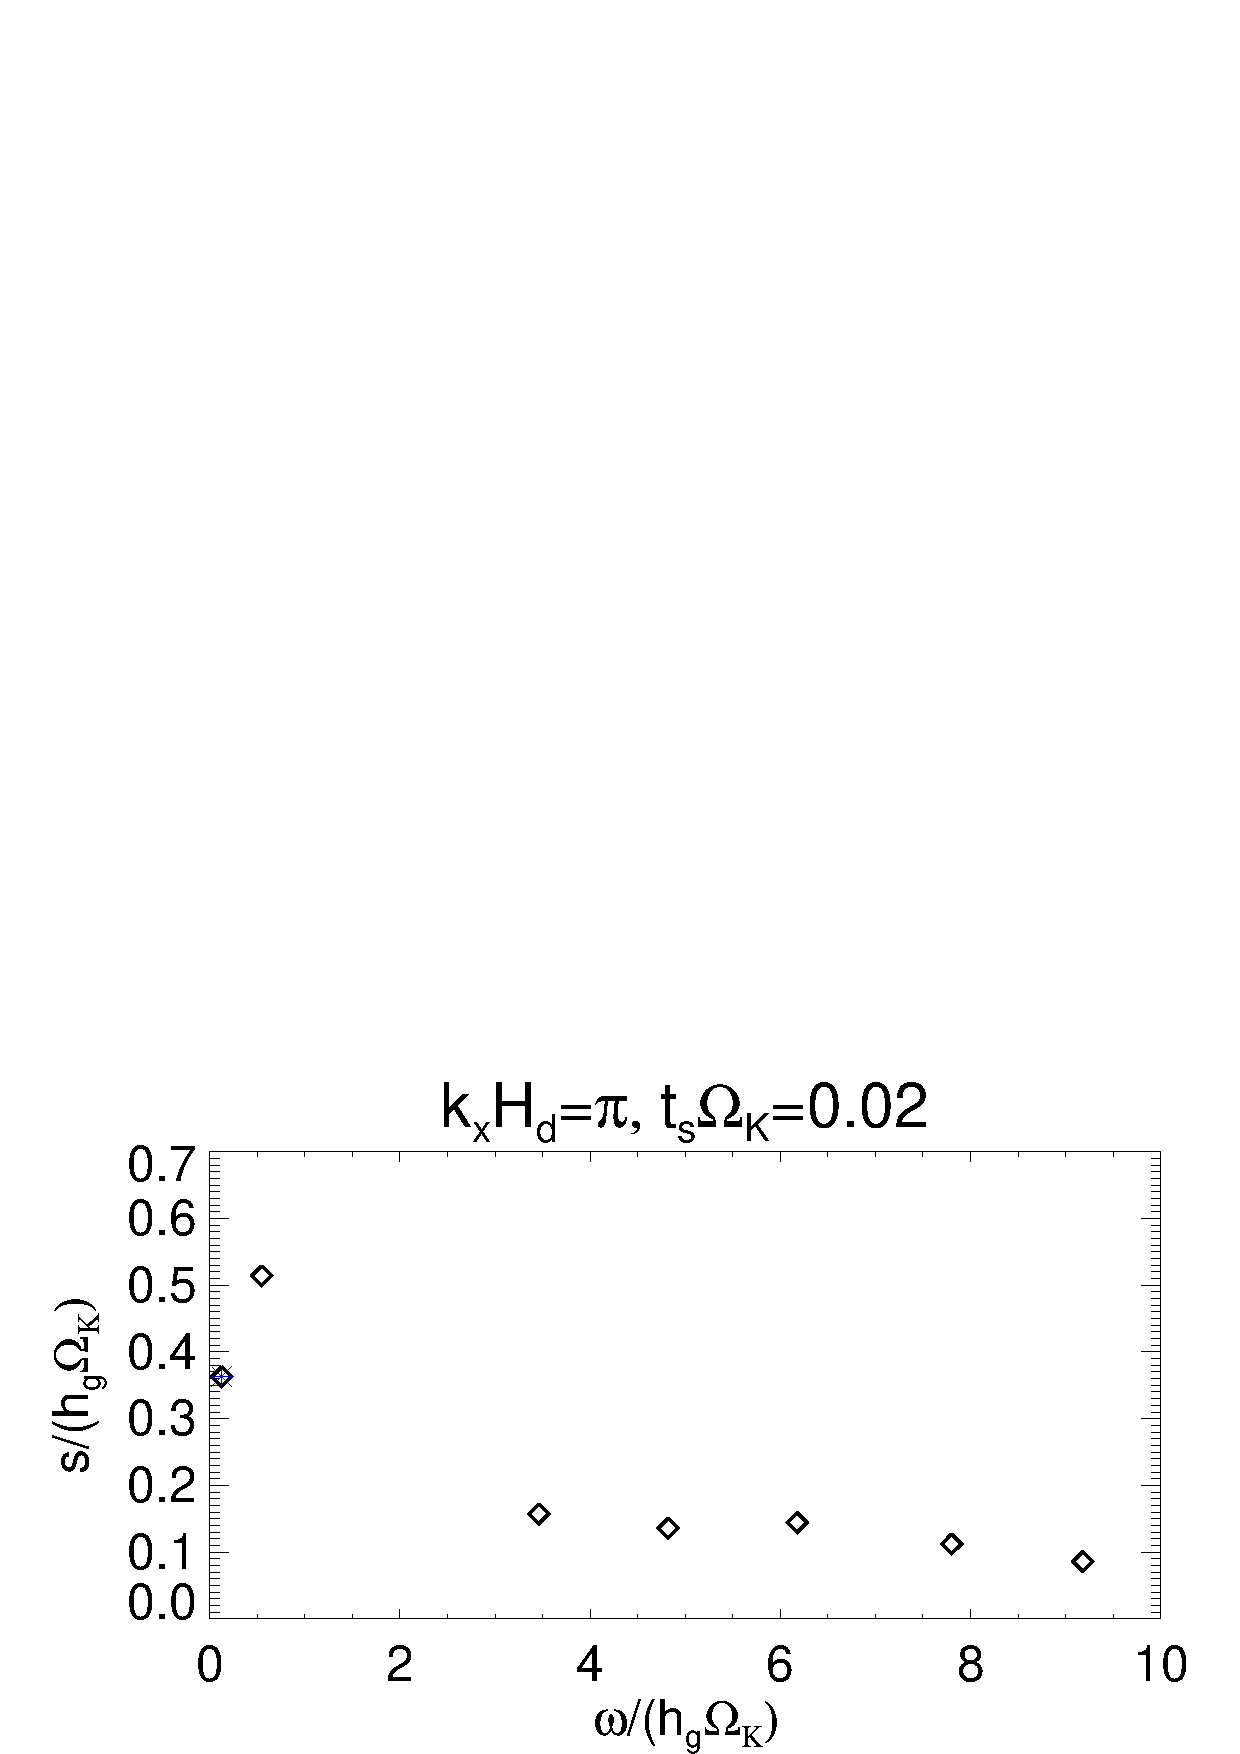
\includegraphics[width=\linewidth]{figures/compare_eigenvals_ts0d02}
%   \caption{Unstable modes in a locally isothermal, dusty disk
%     with stopping time  
%     $\tstop=0.02\OmK^{-1}$. Modes with $\omega>3$ are due to
%     VSI. The mode marked by the blue asterisk, visualized in
%     Fig. \protect\ref{result2d_loren}
%     , is associated with finite dust-gas
%     drag. 
%   }\label{compare_eigenvals_ts0d02}
% \end{figure}


% \begin{figure}
%   \includegraphics[width=\linewidth]{figures/result2d_loren.ps}
%   \caption{Visualization of the mode marked by the blue asterisk in
%     Fig. \protect\ref{compare_eigenvals_ts0d02}. 
%     This is a possible eigenmode of the dusty instability discovered by  
%     \cite{loren15} in their numerical simulations. The instability growth timescale and 
%     radial spacing of the `toroidal vortices' are similar to that 
%     reported by \citeauthor{loren15}. This instability is driven by
%     dust-gas drag. The color scale shows the 
%     perturbed  
%     dust-to-gas ratio, $\delta\epsilon$; and the arrows show
%     $\sqrt{\rho}\left(\dd v_x, \dd v_z\right)$. 
%   }\label{result2d_loren}
% \end{figure}

% One possible interpretation of this mode is `drag-driven VSI', to be 
% compared with `cooling-driven VSI' studied by \cite{lin15}. In the
% latter case, buoyancy forces are eliminated by fast
% cooling, allowing vertical shear to destabilize the disk. Now, in an
% isothermal dusty disk if $\tstop=0$ then mixture is 
% effectively adiabatic: dust-induced buoyancy forces are
% strongest. However, having $\tstop\neq0$ allow dust particles to slip
% past the gas, reducing buoyancy. That is, dust-gas drag
% provies an effective cooling. 

% We stress that this example only serves to highlight
% the possibility of new axisymmetric dust-drag instabilities in
% stratified disks. A major caveat of the above result is that 
% %the base state is not an exact equilibrium, because dust-settling would occur
% %in practice. (
%  the background dust settling timescale is comparable to the instability
% growth timescale. It is essential to construct
% exact equilibria for a meaningful stability analysis. We defer this
% to future work.  

% %also unclear what are "proper" vertical bc for dusty disks 

\section{Summary}\label{summary}
{\bf
In this paper, we examine the conditions under which the presence of
dust can trigger instabilities in gaseous protoplanetary disks.  To this end, 
we develop an analogy between isothermal  dusty-gas and pure ideal
gas. 
} 
The correspondence arises
because drag forces reduce the relative velocity between gas and
dust. In the limit of perfect dust-gas coupling, with stopping time $\tstop \to 0$,  
 dust is entrained in 
the gas. Then the dust-to-gas ratio $\rhod/\rhog$ is conserved
following the flow. This property is analogous to entropy conservation 
following an adiabatic, pure gas. 

For finite drag, $\tstop\neq 0$, the dust content of a 
parcel of the dusty-gas mixture is no longer conserved. The parcel 
can exchange dust particles with neighboring parcels. % owing 
%to dust-gas relative drift. 
This is analogous to heat exchange between a parcel of pure gas and
its surroundings.    

We explicitly show that for a fixed gas equation of state, the  
evolutionary equation for $\rhod/\rhog$ may be replaced by an 
effective energy equation. This leads to a 
natural definition of the effective entropy of isothermal dusty gas as  
\begin{align*}
  \seff  = \ln{\left(\frac{c_s^2\rhog}{\rhog+\rhod}\right)},  
\end{align*}
%This allows us to define the buoyancy frequency of an isothermal 
%dusty gas. 
which implies that a non-uniform dust-to-gas ratio induces buoyancy forces.  
The effect of finite dust-gas friction appears as an energy
source term.  This analogy with standard  
hydrodynamics with cooling/heating allow us to find dusty analogs of gaseous
instabilities, and provide thermodynamical interpretations of  
dust-drag instabilities. 


We obtain the equivalent Solberg-Hoiland criteria for the 
axisymmetric stability of strictly isothermal, perfectly-coupled dusty gas.  
Applying this to typical protoplanetary disks, we find that 
the vertical shear associated with dust 
 layers \emph{cannot} lead to axisymmetric  
  instabilities, however thin the dust layer is.    
Instead, sharp radial  edges in the dust-to-gas ratio could destabilized the
disk, as these imply sharp gradients in the disk's effective entropy
profile. Alternatively, if the dust is vertically well-mixed, then any
radial gradient in $\rhod/\rhog$ can destabilize the disk. 

 % {\bf presumably this limits how sharp dust rings can be} 


We  apply our thermodynamic framework to interpret
the streaming instability \citep[SI, ][]{youdin05a,jacquet11} and to generalize the gaseous vertical shear
instability \citep[VSI, ][]{nelson13,lin15} to dusty disks. We 
explicitly show in SI the evolution of gas 
pressure lags behind dust density. In fact, this is a general property of 
overstabilities driven by dust-gas drag. 
It takes a finite time for the gas to respond to
the dust motion. A lag implies there exists a time interval where 
the gas pressure of a parcel of the dusty-gas mixture is increasing whilst dust is already being expelled.  
The dusty gas then does positive work that amplifies 
oscillations. This interpretation is analogous to stellar pulsational
instabilities \citep{cox67}. 

For the VSI we find dust-loading is generally stabilizing. In our disk models 
dust-loading does not affect VSI growth rates significantly, but
meridional motions may be suppressed where the dust-induced
vertical buoyancy dominates over vertical shear, consistent with our
previous study \citep{lin15}. 
Since the dust-induced buoyancy forces
increase away from the midplane, we find dust-loading can stabilize
`surface modes'  of the VSI, that would otherwise have the largest
growth rates. {\bf We also show that radial variations in
  $\rhod/\rhog$ can trigger a type of VSI, even when the 
  usual sources of vertical shear -- vertical dust gradients and radial 
  temperature gradients -- are negligible.  
  %effectively translates to a non-uniform radial temperature
  %profile, and the resulting vertical shear can lead to instability,
  %even if the true sound-speed is constant. 
}  

%implications for realistic disks
{\bf In a realistic disk, dust particles settle on a timescale $
  t_\mathrm{settle} \sim 1/\tstop\OmK^2$ \citep{takeuchi02}, compared 
  with typical VSI growth timescales, $t_\mathrm{grow}\sim 
  1/h_\mathrm{g}\OmK$. This suggest that particles with $\tstop\OmK\lesssim 
  h_\mathrm{g}$ cannot settle against the VSI. On the 
  other hand, larger particles with $\tstop\OmK\gtrsim h_\mathrm{g}$ should
  settle to form a dusty midplane. In fact, our calculations suggest that
  settling would stabilize the disk against VSI, and allow
  further settling. The result may be a quiet, dusty midplane \citep[unless non-axisymmetric
  instabilities develop, ][]{chiang08} with VSI-turbulent gaseous
  atmospheres. 
}


We also discuss future applications of our thermodynamic framework to 
study dusty protoplanetary disks. Because isothermal dusty gas has an
effective entropy, we suggest that purely hydrodynamic processes, such
as the Rossby Wave Instability \citep{li00} or the `Zombie Vortex
Instability' \citep{marcus15}, where entropy plays a role, could have dusty counter-parts.   
Furthermore, hydrodynamic instabilities driven by thermal cooling, such as VSI in
stably-stratified disks \citep{lin15} or the `Convective
Overstability' \citep{klahr14, lyra14},  may also find dusty analogs 
because finite dust-gas drag is equivalent to a heat sink/source. 

The dusty/adiabatic gas equivalence also offers a simple way to simulate dusty protoplanetary disks 
using purely hydrodynamic codes. All that is required is a re-interpretation of the fluid variables and additional 
source terms in the usual energy equation. The latter is already available in many public codes. In a follow-up work
we will apply this approach to study dusty disk-planet interaction. 


%In particular, we emphasize the 
%physical origin of any instability driven by strong dust-gas
%drag is a phase lag between the pressure and total density evolution
%of the dusty gas mixture. This leads to growing modes because 
%positive work is done during an oscillation cycle, provided by
%dust-gas drag, which is equivalent to a `heat' 
%source. 

%We demonstrate a potentially new dust-drag instability in
%stratified disks that may explain 
 
%We also applied
%our framework to find unstable modes in dusty, stratified disks
%similar to that reported recently by \cite{loren15}. 
